\documentclass[12pt, a4paper]{scrartcl}
\usepackage[english]{babel}
\usepackage{natbib}
\usepackage{url}
\usepackage{lmodern}        % Latin Modern family of fonts
\usepackage[T1]{fontenc}    % fontenc is oriented to output, that is, what fonts to use for printing characters. 
\usepackage[utf8]{inputenc}
\usepackage{amsmath}
\usepackage{amssymb}
\usepackage{graphicx}
\graphicspath{{../figs/}}
\usepackage{subcaption}
%\usepackage{parskip}
\usepackage{fancyhdr}
\usepackage{vmargin}
\usepackage{hyperref}
\usepackage{cleveref}
\usepackage{csquotes}
\usepackage{bm}
\usepackage{placeins}
\usepackage{pdfpages}
\usepackage{blindtext}
\usepackage[list-final-separator={, and }]{siunitx}
\usepackage{mathtools}

%\setmarginsrb{3 cm}{2.5 cm}{3 cm}{2.5 cm}{1 cm}{1.5 cm}{1 cm}{1.5 cm}
\setmarginsrb{3 cm}{1.5 cm}{3 cm}{1.5 cm}{1 cm}{0.5 cm}{1 cm}{0.5 cm}
\title{Breast Cancer Wisconsin Data Set} % Title
\author{Jannik Lukas Kossen \& Ahmad Neishabouri}                               % Author
\date{\today}                                         % Date

\makeatletter
\let\thetitle\@title
\let\theauthor\@author
\let\thedate\@date
\makeatother

\pagestyle{fancy}
\fancyhf{}
\rhead{\theauthor}
\lhead{Fundamentals of Machine Learning}
\cfoot{\thepage}

% Fix BibTex error
\setcitestyle{numbers}

% Define argmin, max
\DeclareMathOperator*{\argmin}{arg\,min}
\DeclareMathOperator*{\argmax}{arg\,max}
\DeclarePairedDelimiter\norm{\lVert}{\rVert}

\begin{document}

%%%%%%%%%%%%%%%%%%%%%%%%%%%%%%%%%%%%%%%%%%%%%%%%%%%%%%%%%%%%%%%%%%%%%%%%%%%%%%%%%%%%%%%%%

\begin{titlepage}
    \centering
%    \vspace*{0.5 cm}
    
\includegraphics[scale = 0.6]{hdlogo}\\[2.0 cm]  % University Logo
     \begin{flushleft}
     \large  \hspace{1cm} A report on the 
	\end{flushleft}      
     \centering
    \rule{\linewidth}{0.2 mm} \\[0.4 cm]
    { \huge \bfseries \thetitle}\\
    \rule{\linewidth}{0.2 mm} \\[1.5 cm]
    
    \textsc{\LARGE Final Project}\\[0.5 cm]               % Course Code
    \textsc{\Large Heidelberg Collaboratory \\[0.5em] for Image Processing}\\[2.0 cm]  % University Name
    \thedate
   	\\[3em]
    \large
            \emph{Submitted to:}\\[1em]
            PD Dr.\ Ulrich Köthe \& M.\ Sc.\ Lynton Ardizzone\\[1cm]
            \emph{Submitted by:} \\[1.5em]
            \begin{minipage}{0.4\textwidth}            
            	\begin{flushleft} 
					\large Jannik Lukas Kossen (JK) Student ID: 3495228 \\
					\small M.Sc. Physics, ungraded\\
      		  \end{flushleft}
      		 \end{minipage}
            \begin{minipage}{0.4\textwidth}            
            	\begin{flushright} 
    	    	    \large Ahmad Neishabouri (AN) Student ID: 3436580 \\ 
         	   		\small M.Sc. Scientific Computing, graded
      		  \end{flushright}
      		 \end{minipage}\\[2 cm]


        
 
\end{titlepage}


\tableofcontents
\pagebreak




%TODO fix titlepage (names and everything) 
%TODO centralise for PCA! dont normalise necessarily
%TODO reread algorithms in barbers book
%TODO figure out if imbalance is a problem
%TODO  put this in?
% Validation data is only needed when we compare different models. The cross validation might just yield a "lucky" winner. (Using different models on the test set can be seen as overfitting the test set. The winning model might have just been lucky. 


% How to include a figure.
%\begin{figure}
%	\centering
%	
\includegraphics[width=0.7\textwidth]{hdlogo}
%	\caption{A figure.}
%	\label{fig:class-incremental}
%\end{figure}

\section{Introduction (JK)}
The following pages contain the report on our final project for the \emph{Fundamentals of Machine Learning} lecture given by PD Dr.\ Köthe in the last semester. As the lecture focused on the \emph{fundamentals} of machine learning, we see this project as an opportunity to explore and revise again some fundamental techniques of machine learning and also dive into some of the algorithms which, while they were presented in the lectures, were not discussed in the tutorials.  Often, the application potential of these basic techniques on real-world tasks is rather small. However, they do constitute the foundation of more recent and better algorithms, which often embed or build upon these methods. 

The focus of this project shall therefore not be to \emph{solve} a task using fundamental machine learning, but rather to carefully study the different algorithms and compare their strengths and shortcomings in comparison with each other. To narrow the focus of the project a bit, we have chosen to only compare \emph{classification} methods.
We work with the \emph{Breast Cancer Wisconsin (Diagnostic) Data Set} \cite{street1993nuclear}, a binary classification task with the aim to identify whether a person does or does not have breast cancer based on a set of hand-crafted features. The data set should work well for benchmarking algorithms, providing a nice balance between being well-behaved, i.e.\ solvable, and possessing enough depth and character to allow for some comparison between the algorithms, i.e.\  not being trivial to solve.


\paragraph{Data Set.} The abovementioned data set was first published alongside a paper called \emph{Nuclear Feature Extraction For Breast Cancer Diagnosis} \cite{street1993nuclear} in the 1993 edition of the \emph{International Symposium on Electronic Imaging: Science and Technology}, wherein a classification pipeline for breast cancer diagnosis is proposed. A small sample of skin tissue is extracted from the patients breast and analyzed using a camera mounted atop a microscope. Using an interactive tool the operator identifies individual cell nuclei, whose outlines are then semi-automatically determined. For each nucleus, ten features that are sought to describe the geometric shape and appearance of the nucleus are crafted. These features are the radius, perimeter, area, compactness, smoothness, concavity, concave points, symmetry, fractal dimension, and texture of the nucleus.
For the sake of brevity, the reader is referred to the original publication \cite{street1993nuclear} for a detailed description of how these features are calculated from the image and outline of a nucleus. 
The mean, extreme, and standard deviation values of these features are then calculated for the nuclei of a single sample, giving, in total, a 30-dimensional feature vector describing each sample.
The hope here is obviously, that these features (or a subset thereof) capture the differentiating aspect of tumor-ridden cell nuclei from their healthy counterparts. The data set is explored further in \cref{sec:expe}.

\paragraph{Structure.} The structure of this report is as follows: \cref{sec:theo} discusses the theoretical foundations of each of the compared methods. In \cref{sec:expe}, unsupervised exploration techniques are employed to gain some understanding of the shape of our data set. The classification methods are applied, benchmarked and investigated. \Cref{sec:discu} then expans on the discussion of these results in relation to peculiarities of each method and the data set. Finally, \cref{sec:sum} gives a summary of this report.

As demanded by the faculty of Mathematics and Computer Science, each section or paragraph heading also contains a shorthand symbol, \emph{(JK)} or \emph{(AN)}, to indicate whether a certain section was written by Jannik Kossen or Ahmad Neishabouri.

\section{Theoretical Background}	
\label{sec:theo}

\paragraph{Preliminary Remarks (JK).} Note that, unless marked otherwise, for clarity, the theoretical derivations follow the lecture \cite{kothe2018foml} in content and notation.
This includes the convention to describe the data as $X = ( X_1, X_2, \dots, X_N)$, where $N$ is the number of instances and each $X_i$ is a $D$-dimensional feature (row) vector. The feature $j$ of instance $i$ is therefore given by $X_{ij}$.  Index $i$ is solely used to index along the $N$-dimensional instance axis, whereas $j$ solely indexes the $D$-dimensional feature axis. The labels or ground truth instances of supervised learning are given as $Y_i$.


\paragraph{Logistic Regression (AN). }  Against what the name may imply, logistic regression is a model used for classification problems, in which it models the probability that the response belongs to a particular category. Applying simple linear regression model to guess such probabilities may lead to probabilities outside 0 and 1 interval, which makes it hard to interpret as probabilities.
To avoid such problems, probabilities should be calculated using functions that result in a [0, 1] interval. For logistic regression, logisitic sigmoid functions is used in lecture notes:
\begin{align}
	\sigma(t) = \frac{1}{1 + \exp(-t)}
\end{align}

The distinct property of the sigmoid function, which is also known as \emph{squashing function}, is that it maps the whole real line result to a 0 and 1 range, as we asked for. By implementing the above model in a Maximum Likelihood method, we'll be able to fit the model.

\paragraph{Principal Component Analysis (JK).} Principal Component Analysis (PCA) is a simple yet effective dimension reduction technique. Often, it is also used exploratively to gain an understanding of the complexity of a data set. In PCA, one aims to map instances $X_i$ of the original feature space $\mathbb{R}^D$ to features $Z_i$ in a lower-dimensional feature space $\mathbb{R}^{D^\prime}$ via a linear mapping
\begin{align}
	Z_i = X_i A + b \, 
\end{align}
where $A$, a $D\times D^\prime$ matrix, and $b$ are the parameters of the linear mapping. We now define a mapping from $\mathbb{R}^{D^\prime}$  back to the original space $\mathbb{R}^D$ as
\begin{align}
	\tilde{X}_i = V Z_i + \mu \, ,
\end{align}
where for the sake of simplicity we assume $D^\prime=1$ in the derivation without loss of generality.
The ideal linear mapping between the two feature spaces is now found by demanding that the squared loss between the original $X_i$ and the reconstruction $\tilde{X}_i$ is minimized
\begin{align}
	\argmin_{V, \mu, \{Z_i\}} \: \sum_i \left( X_i - \tilde{X}_i \right)^2 \, .
\end{align}
By requiring centralized data $\bar{X}=0$, setting the arbitrary $\bar{Z}=0$, and requiring normalized $V^TV$, one finds the simplified version (see lecture for full derivation)
\begin{align}
	&\argmin_{V, \{Z_i\}} \: \sum_i ( X_i - 
														\underbrace{V Z_i}_{\mathclap{=(X_i V^T)V}}
														)^2 \quad
														\text{s.t.} \enspace V^TV=1  \\
	&\argmax_{V, \lambda} \: VSV^T + \lambda \,  (1-VV^T) \, ,													\end{align}
where $\lambda$ is the Lagrange parameter for the constraint on $V$ and $S$ is the scatter matrix $S = \sum_i X_i^T X_i$. 
The derivation is presented in such detail here, because an important insight can be gained  by deriving the above expression w.r.t. $V$, giving
\begin{align}
	S V^T = \lambda V^T \, .
\end{align}
$V^T$ is an eigenvector of S. Substituting this into the above problem simply yields
\begin{align}
	\argmax_\lambda \lambda \, .
\end{align}
The projection problem therefore has been reduced to finding the biggest eigenvector of S. In other words: if we want to linearly project our data into a one-dimensional feature space while retaining maximal information, we project along the direction of $V$, the vector belonging to the biggest eigenvalue $\lambda$ of the scatter matrix. Similarly, if we want to transform to a $D^\prime$ dimensional feature space, we project the original data instances along the $D^\prime$ largest eigenvectors $V_j$. Given by the optimization constraint above, the features (eigenvectors) of the new space are orthogonal. 

It can be shown that the projection vectors $V_j$, sorted by their eigenvalue size, project the data along those orthogonal axes that lie along the direction of maximal variance in the original space $\mathbb{R}^D$. This is because axes with a high variance contain a lot of information and therefore minimize said information loss when transforming to the new, lower-dimensional feature space.
\paragraph{Linear Discriminant Analysis (AN).} Another method commonly used for dimensionality reduction is Linear Discrminant Analysis(LDA), however, in contrast to previously described method of PCA, LDA is \emph{supervised} and which tries to find the axes direction with maximum between classes separation.

\begin{figure}
	\centering
	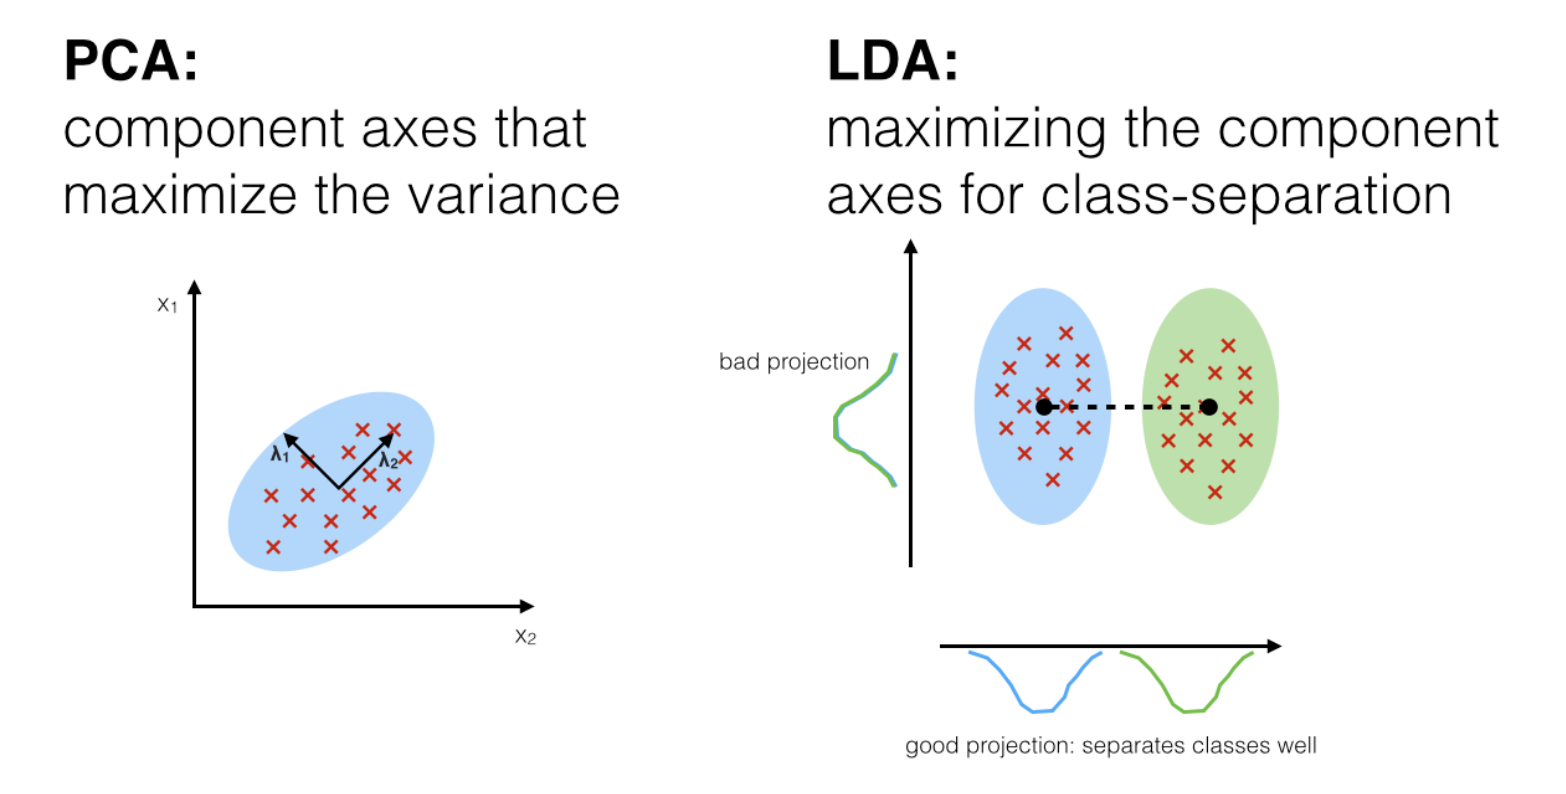
\includegraphics[width=0.7\textwidth]{LDAvsPCA}
	\caption{LDA vs PCA. Image Credit \citep{raschka2014linear}}
	\label{fig:LDAvsPCA}
\end{figure}

However, we are using LDA here as a classification method, in which we are trying to best separate classes from each other. Comparing LDA to Logistic Regression, Logisitc regression tries to directly model $Pr(Y = y | X = x)$ using logistic function(Discriminative Model), while one can first model the distribution of the predictor X, separately in each of the response classes Y, and then using Bayes' theorem to estimate  $Pr(Y = y | X = x)$ (Generative Model). While there is high similarity between the Logistic Regression Model and LDA models for normal distributed instances, one aim to perform an LDA for the following reasons\cite{James:2014:ISL:2517747}

\begin{description}
  \item[$\bullet$] Well separated classes result in an unstable parameter estimation in Logistic Regression
  \item[$\bullet$] LDA is more stable when the number of instances are small and the distribution of $X$ is normal.
  \item[$\bullet$] LDA is highly popular when we are dealing with more than two response classes.
\end{description}

While in this project only the second reason might motivate us, however we did apply an LDA classification to compare with other methods. Linear Discrminant Analysis is derived as explained above, by first assuming a multivariate Gaussian distribution with a class specific mean vector and with constant covariant matrix for all classes. This means that we are assuming that all the clusters have the same elliptic shape and size. By maximising the likelihood of the training set(details in lecture notes \citep{kothe2018foml}), we would result to the following classifier:

\begin{align}
	\hat{k} = \argmax_{k}W^{T}_{k} . x + b^\prime_{k}
\end{align}

in which:

\begin{align}
	W^{T}_{k} = 2 \mu^{T}_{k}\Sigma^{-1}
\end{align}

is derived by fitting a Gaussian distribution to within class covariance.

\paragraph{Quadratic Discriminant Analysis  (AN).} Qudratic Discriminant Analysis (QDA) follows the same steps as in LDA, in which it results from assuming that all observation are drawn from a Gaussian distribution, and using the Bayes' theorem to estimate the parameters to perform prediction. However, in contrast to LDA in which places a constant covariance matrix to each class, QDA assumes that each class has a different covariant matrix. This would result in a more complex model, thus in more parameters to be estimated. in addition, LDA is much less flexible than QDA which would result in less variance. However, the trade-off is when the K classes are actually does not share a common covariance matrix, which then would result in a high bias. Therefore, LDA would be better choice than QDA if the training set is small and reducing variance is crucial. 

By maximising the likelihood of the training set, and assigning a separate covariance matrix for each class, we would result in

\begin{align}
	\hat{k} = \argmin_{k}(x - \mu_{k})^{T}\Sigma^{-1}_{k}(x - \mu_{k}) + b_{k},
\end{align}

which is a \emph{quadratic} function of $x$. 

\paragraph{(k-)Nearest Neighbor Classification (JK).} One of the simplest approaches to classification is the the nearest neighbor (NN) classifier. Test set instances $i$ are simply classified with the same class as their \emph{nearest} neighbor from the training set (TS). 
Which neighbor is \emph{nearest},  is given by some distance metric $d(X_i, X_{i^\prime})$ between to instances $X_i$ and $X_{i^\prime}$. $d(X_i, X_{i^\prime})$ is often chosen to simply be the Euclidean distance.
In mathematical terms, the decision function for the NN classifier can be written as
\begin{align*}
	f_{\mathrm{NN}} = Y_i \, \text{,  where } \, i = \argmin_{i^\prime \in \mathrm{TS}} \: d(X_i, X_{i^\prime}) \, .
\end{align*}
The NN classifier requires the total memorization of the training set which becomes problematic for larger data sets.
A simple variant of the NN classifier is the k-nearest neighbor algorithm, which classifies instances by taking a majority vote of the classes of the surrounding k-nearest neighbors of the instance that is to be classified. In contrast to the simple NN classifier, the k-NN classifier is consistent, i.e.\  the k-NN classifier converges to the optimal Bayes classifier as $N\to\infty$.

\paragraph{Decision Trees (AN).} Very much similar to a 20 questions game, a series of questions will result in a decision trees model which would be implemented for classification and regression tasks. In case of data with continuous features, as it is the case most of the time in data science, these questions would take the form of "Is feature i larger that value a?" \citep{muller2016introduction}

The series of if/else questions asked in decision trees are called \emph{tests} and the algorithm is learned to ask the most informative questions in regard to the target values. These tests will split the data set, or the so called \emph{root node}, in each step to two nodes. The first layer nodes would mostly contain targets from each class, but the more deep one would go in asking questions, the more complex the model would become and the more \emph{pure} the terminal nodes (referred to as \emph{leaves}, and located at the bottom of the tree) would become. Since these segmenting and splitting of the data set can be summarized in a tree, these method are know as \emph{decision tree} models.

Prediction is performed by first dividing the predictor space into $\mathcal{J}$ distinct and non-overlapping regions $\mathcal{R}_{1}, \mathcal{R}_{2},..., \mathcal{R}_{\mathcal{J}}$ in a \emph{top-down}, \emph{greedy}\footnote{greedy because in each step it only tries to find the best split on the current step, regardless of how another split may result in more information in future steps.} approach, and then for each instance in test set, we'll investigate in which region $\mathcal{R}_{i}$ will the instance fall into \citep{James:2014:ISL:2517747}. The prediction then will be the class assigned to region $\mathcal{R}_{i}$, in classification tasks, or the mean of the response values of training set in region $\mathcal{R}_{i}$, in regression tasks.

Decision trees are pretty much prone to over-fitting by asking too much questions. Such models would result in a pretty much pure leaves and high accuracy on training set, but poor performance on test sets. Two major strategies would be recommended to take in such cases to reduce the variance on the training set. First would clearly be asking less questions, resulting in smaller trees with fewer splits, and fewer regions $\mathcal{R}_{1}, \mathcal{R}_{2},..., \mathcal{R}_{\mathcal{J}}$. This approach is also called \emph{pre-pruning} and can be implemented in different ways, one would be by introducing a threshold to how informative are the questions and stop whenever there is no question that would result a changes higher (or lower) than the threshold. \footnote{a rather short-sighted approach because of the tree making process being greedy, which will result in early stoppage of the process} Other method would simply be stopping the method after certain number of questions in a certain depth. The second strategy would be to grow a large tree at first and then \emph{prune} the leaves with less or no information to obtain a \emph{subtree}. 

Decision trees have the advantage of being simple to explain, simple to display graphically, and more over, there is no need to do any preprocessing like normalization or standardization of features and that is because the algorithm is invariant to scaling of the data. However, this method has shown high tendency to being over fit even with applying pre-pruning to it. This is why ensemble methods of using multiple trees explained in next section is usually  used in such applications. In \cref{sec:expe} we'll apply decision trees on the data set with pre-pruning parameters as a tuning parameter to find the best bias-variance trade off. 


\paragraph{Random Forests (AN).} Ensemble methods apply different machine learning models together resulting in models with better performance. Of these ensemble methods, Random Forests showed to be effective in both Classification and regression tasks. Random Forests basically uses decision trees as the building blocks for the model. As we mentioned in previous section, the main disadvantage of decision trees is that it tends to overfit to training data and they don't have good predictions on test set. However, in random forest we try to overcome this by the ensemble of different trees together and the concept is as follows: Each tree will try to predict a certain target but it would overfit in certain direction, however applying many of them and averaging the results would lower the overfitting and maintaining the same prediction results, a process know as \emph{decorrelation} of trees. 

There are other methods in which they implement number of decision trees in their model, like \emph{bagging} or \emph{boosting}, however random forests are different in which they introduce randomness in their tree building process to make sure that each tree does a different task and is different. This process is ensured by combining two different random process: first is the random selection of data points, and second is random selection of the features.

This process is starts by building a number of decision trees on \emph{bootstrapped} training samples. Bootstrapped samples are made by drawing samples from the set in random and allowing the samples to be repetitive. This will result in data set as big as the main data set, with some data being missed, and some of them being repeated. After making bootstrapped samples on the original data set, here comes the second random process, the random feature selection, and it works as follows: we start to build the decision trees on the bootstrapped sample, however this time, we'll limit the process of finding the best feature for each test to a certain group of random chosen features set, and this random feature selection is repeated on each and every node built in tree. 



\paragraph{Support Vector Machine (JK).} Out of all of the presented algorithms in the lecture, Support Vector Machines (SVMs) are among the most powerful and widely used. Similar to the previously presented linear discriminant analysis / logistic regression, in SVM, decision planes are trained to discern between positive and negative instances of the data. When the data is linearly separable, i.e.\  there are multiple hyperplanes that perfectly separate the different classes, SVM chooses that hyperplane which maximizes the so-called \emph{safety margin}
\begin{align}
	\max_{\beta, \beta_0} M = 	\max_{\beta, \beta_0} \left\{ \min_i Y_i ( X_i \beta + \beta_0) \right\} \, .
\end{align}
$X_i \beta + \beta_0$ gives the signed distance of instance $X_i$ to the decision plane parametrized by $(\beta, \beta_0)$. $Y_i (X_i \beta + \beta_0)$ is always positive. 
We therefore find the decision plane by maximizing the margin for the points closest to the decision plane. The obtained solution for an SVM depends entirely on those critical points, i.e.\  the decision plane of an SVM is governed by the points close to the decision plane, completely unlike the abovementioned LDA, where the majority of the points, which are close to the mean and not the boundary, decide the position of the plane. 

Setting the arbitrary $M=1$ and rescaling by the norm of $\beta$ yields the optimization problem of the linear SVM for separable data
\begin{align}
	\hat{\beta}, \hat{\beta_0} = \argmin_{\beta, \beta_0} \,  \norm{ \beta}^2 
	\quad \text{s.t.} \enspace \forall i: Y_i (X_i \beta + \beta_0 \ge 1) \, ,
\end{align}
where the constraint ensures that the plane strictly separates data of the two classes.
Since real world data are usually not linearly separable, so-called \emph{slack} variables $s_i$ are introduced that represent a trade-off between the maximization of the margin and minimizing the loss over the training instances. 
By rearranging the constraint the linear SVM can be rewritten as
\begin{align}
	\hat{\beta}, \hat{\beta_0} = \
	min_{\beta, \beta_0} \,  \frac{1}{2} \, \norm{ \beta }^2 + \frac{C}{N}\, \sum_i \text{loss} (X_i, Y_i | \beta, \beta_0) \, ,
\end{align}
where $C$ now represents the trade-off parameter between the two objectives. Ideal $C$ can be found using cross-validation. In SVM we also get to chose a loss term, a popular choice being the \emph{hinge loss}
\begin{align}
	\text{Hinge Loss }(\hat{Y}_i, Y_i) =  \max(0, 1-\hat{Y}_i  Y_i) \, .
\end{align}
However, other types of losses are possible, with most popular choices producing comparable outcomes, as they behave similarly near the decision boundary.
From the above expression, a dual formulation can be obtained which is suited for a kernelized version of the SVM, not derived here.
Suffice to say, that to get to a kernel SVM, the above optimization problem has to be reformulated such that the data is only accessed via scalar products $X_i^T X_i^\prime$ which are then replaced by a kernel function $K(X_i, X_i^\prime)$. This introduces a non-linearity that effectively maps the data to a higher-dimensional space and allows one to solve more complex problems at the cost of introducing additional hyperparameters.
A popular kernel choice is the Gaussian kernel
\begin{align}
	K(X_i, X_i^\prime) = e^{-\gamma \norm{ X_i - X_i^\prime }^2} \, 
\end{align}
although other kernels such as polynomial or sigmoid kernels are also used.

The SVM optimization problem can be solved iteratively using various gradient descent methods.%

\paragraph{Multilayer Perceptron (JK).} Even though they were not part of the lecture, it seems wrong to not discuss neural networks at all. They have been hugely successful within the machine learning community, finding application in a broad variety of topics. While a lot of research in computer vision is dedicated to \emph{convolutional neural networks}, simple neural networks can also be employed to do classification tasks.
This is why, even though cutting-edge neural networks are not discussed here, the multilayer perceptron (MLP), a basic artificial neural network achitecture, is introduced and applied. A \emph{very} brief description is given in the following paragraph, for a more detailed description see e.g.\ \cite{bishop2006prm}.
An MLP, as depicted in \cref{fig:mlp}, consists of several connected layers, themselves consisting of a column of neurons. Each neuron receives an input signal that is a weighted sum over all of the outputs of the neurons in the previous layer. A so-called bias is added to that sum and finally, a non-linearity is applied to give the output of that neuron.
A common non-linearity is the ReLU (rectified linear unit) function, defined as $\max(0, x)$.
 The output $o_{1i}$ for a neuron $z_{1i} $ in the first hidden layer would be
\begin{align*}
	o_{1i} = \text{sigmoid}\left( W_{1i} \, z_{0} + b_{1i} \right) \, ,
\end{align*}
where $W_{1i}$ are the weights connecting the inputs  $z_{0}$ to the neuron $i$ in the first hidden layer and $b_{1i}$ is the bias term. This way, information propagates through the network from the input layer to the outputs. Any neural network therefore is a nested application of non-linear functions of the input data.

\begin{figure}
	\centering
	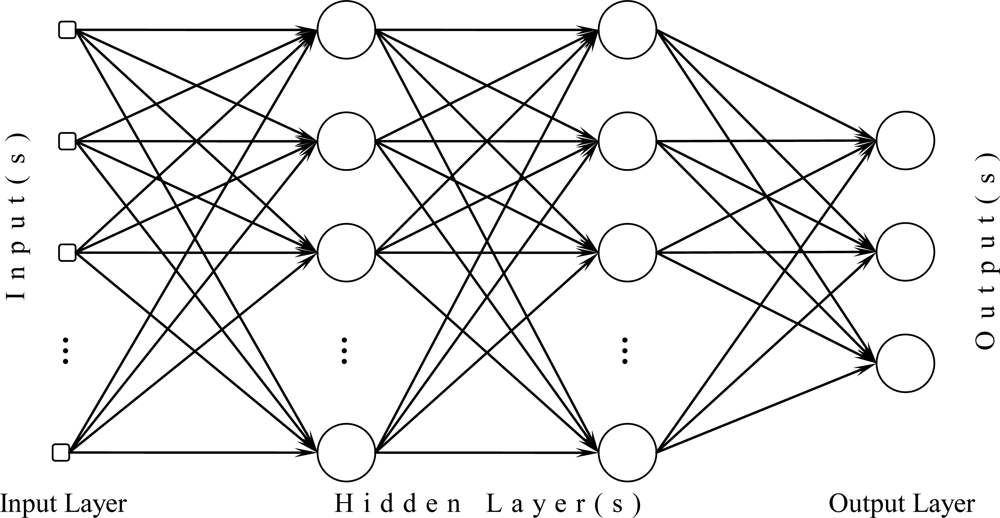
\includegraphics[width=0.7\textwidth]{mlp}
	\caption{Schematic diagram of a MLP. Image Credit \citep{saracoglu2010color}.}
	\label{fig:mlp}
\end{figure}

For the binary classification problem at hand, the output layer consists of two nodes, one for each of the classes. In training, the neural network is presented with examples from the training set and the output from the last layer is compared to the ground truth labels. For binary classification problems, a binary cross entropy loss, similar to LDA,
\begin{align}
	\text{Loss}\, (\{y_i, \hat{y_i}\}) = \frac{1}{N_b} \, \sum_{i=1}^{N_b} \left( y_i \log(\hat{y_i}) + (1-y_i)) \log(1-\hat{y_i}) \right)
\end{align}
is used. Here, $N_b$ is the batch size which is not necessarily equal to the number of instances $N$ in the data set. This loss can then be minimized in training, by means of \emph{backpropagation}: the partial derivatives of the loss with respect to the parameters are calculated and the parameters adjusted accordingly to minimize the loss.
Through many iterations of this, the network can be fit to the data set, although one needs to be careful not to overfit to the data.
Early stopping (stop the training process before convergence) and regularization techniques such as dropout (randomly drop a proportion of the neurons from the network)) may be used to combat overfitting.

\section{Experiments \& Discussion}
\label{sec:expe}
In the following, the tools and implementations from the python library scikit-learn \cite{scikit-learn} are heavily used. For the multilayer perceptron, the popular library tensorflow \cite{tensorflow2015-whitepaper} is employed.

\subsection{Exploratory Analysis \& Introduction to the Data Set (JK)}
Before the introduced classification methods are applied, it is crucial that some time is spent on exploring the \emph{Breast Cancer Wisconsin Data Set}.
The data set consists of $N=569$ instances with $D=30$ feature dimensions. The data are somewhat imbalanced as \SI{63}{\percent} of the instances are false, i.e.\  come from benign cells without breast cancer. This might have to be accounted for in the analysis.
Data will be centered and standardized according to the training set distribution unless otherwise mentioned.
To get a feeling for the data, 16 random combinations of two dimensions of the data set are shown in a scatter plot in \cref{fig:random_scatter}. While for some features, the different classes are clumped together, we can already see that for others, a separation and therefore successful classification might be possible.

\begin{figure}
	\centering
	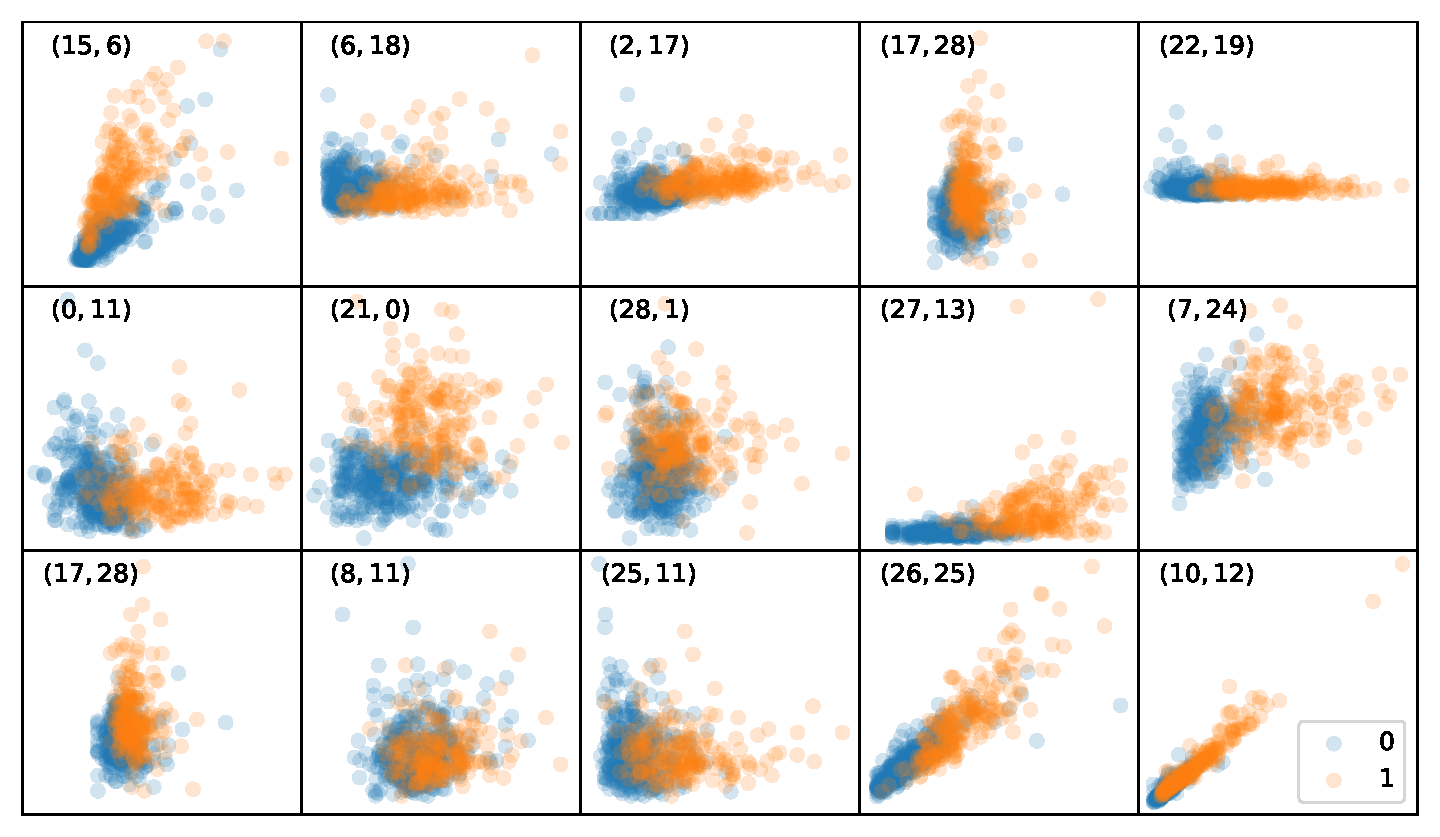
\includegraphics[width=\textwidth]{random_scatter}
	\caption{Shown are random 2D slices of the data set. Given in parenthesis are the dimensions that give the $(x,y)$ axis of the scatter plot.}
	\label{fig:random_scatter}
\end{figure}

Following this hunch, a continued investigation of the data set is therefore pursued via PCA.
The results of the PCA are given in \cref{fig:pca}. We can see that the linear PCA is already fairly successful at separating the different classes in the data. Note, that as PCA is an unsupervised method, it has not been given any labels, which are only shown for clarity. In \cref{fig:pca1} one can see that just by projecting the data among axes of high variance, the two classes are somewhat separated. \Cref{fig:pca2} shows that the projection vectors actually point along axes of high variance in the original space. Note, that the two vectors being shown here only \emph{seem} to note be orthogonal, due to the fact that a 2D slice of the 30 dimensional feature space is shown. Finally, \cref{fig:pca3} shows that the first component of the PCA can almost explain \SI{50}{\percent} of the variance in the data, if the first 6 components are combined this rises to \SI{90}{\percent}. 
The dimensions in \cref{fig:pca2} were chosen as the highest contributors to the first component of the PCA, which is why they also exhibit a high variance.

\begin{figure}
    \centering
    \begin{subfigure}[b]{0.3\textwidth}
        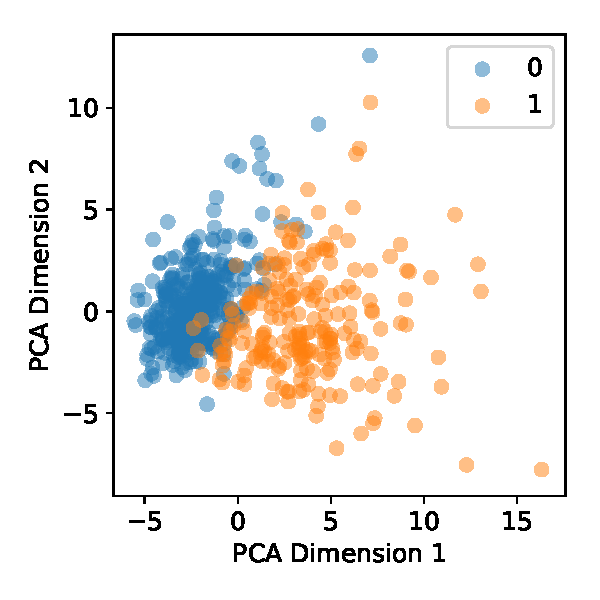
\includegraphics[width=\textwidth]{pca_1}
        \caption{}
        \label{fig:pca1}
    \end{subfigure}
    \begin{subfigure}[b]{0.3\textwidth}
        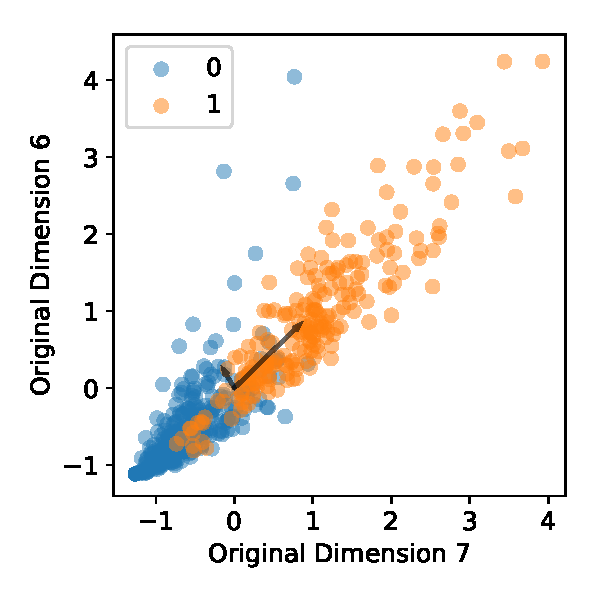
\includegraphics[width=\textwidth]{pca_3}
        \caption{}
        \label{fig:pca2}
    \end{subfigure}
    \begin{subfigure}[b]{0.3\textwidth}
        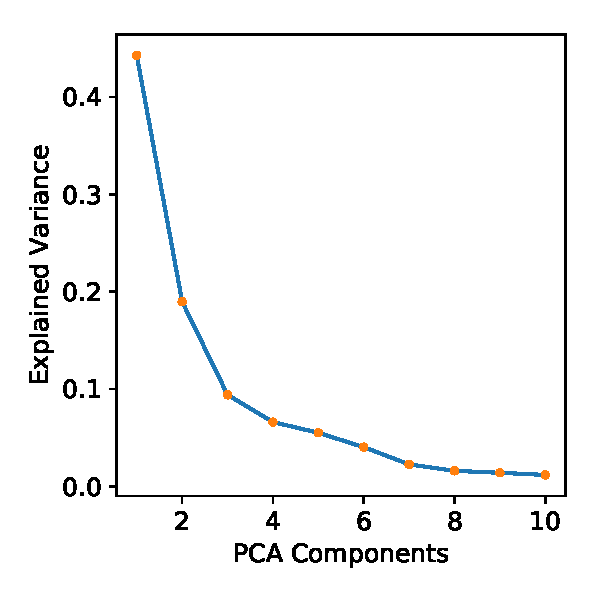
\includegraphics[width=\textwidth]{pca_2}
        \caption{}
        \label{fig:pca3}
    \end{subfigure}
    \caption{PCA of the data set: (a) shows the two most important dimensions of the data set in the transformed space, (b) shows how the PCA projects along axes of maximal variance in the original space, where the arrows indicate the direction of projection, and (c) shows the explained variance of the original data set per PCA component.}\label{fig:pca}
\end{figure}

In conclusion, PCA can be successfully applied to this data set as a dimensionality reduction technique. The transformed, lower-dimensional data can then be used as an input to other classification algorithms. The success of the linear PCA also shows that the complexity of the data set is somewhat limited and that we can expect successful results from the basic classification methods presented in the lecture.

\subsection{Classification Algorithms}
\paragraph{Evaluation (JK).} In order to provide reliable performance analysis, 10-fold cross-validation is employed for each algorithm. A strict separation of training and test set is ensured such that meaningful statements over the predictive power of the methods can be made.
Whenever an algorithm has hyperparameters an exhaustive grid search is performed in order to find the best-performing set of parameters. \emph{Performance} is given in terms of accuracy and or precision-recall curves. 

\paragraph{Logistic Regression (AN)} In Logistic Regression, the trade-off parameter for assigning the strength of regularization is tuned by changing the C parameter, in which higher values of C correspond to less regularization. This parameter works in a way that penalizes large weights which will result in reducing the flexibility of fitting the training data, and hence having better performance on test data.

We started by implementing the logistic regression classifier on the data set for different C parameters trying to find the best value for this parameter. \cref{fig:logistic_regression} shows the precision-recall plot for the test set. 


\begin{figure}[h]
    \centering
    \begin{subfigure}{0.45\textwidth}
        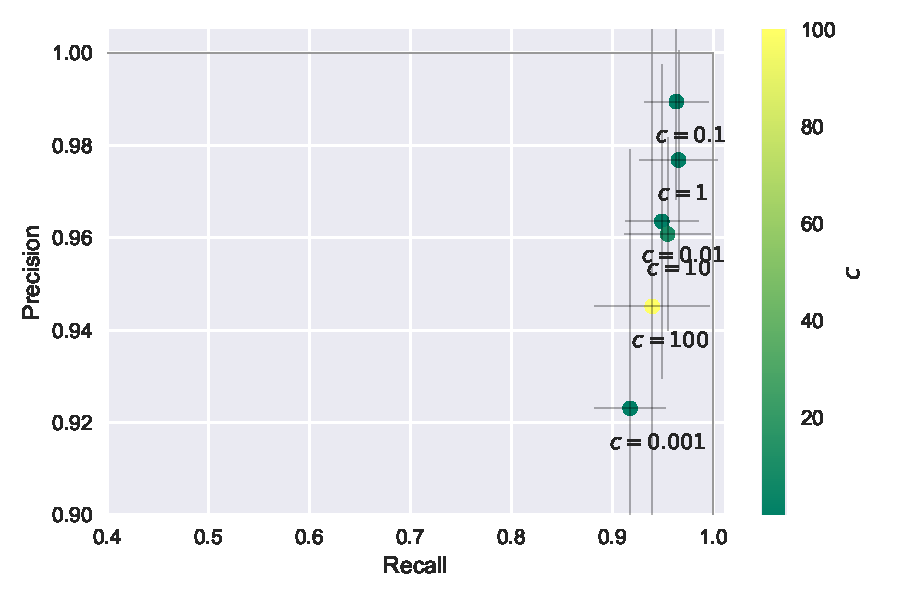
\includegraphics[width=\textwidth]{logistic_regression}
        \caption{}
        \label{fig:logistic_regression}
    \end{subfigure}
    \begin{subfigure}{0.45\textwidth}
        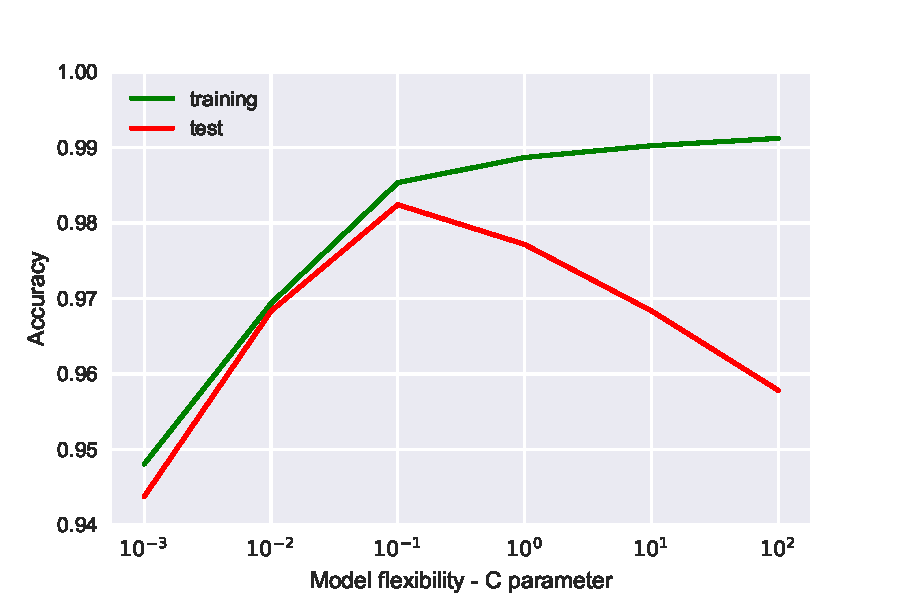
\includegraphics[width=\textwidth]{tradeoff_lr}
        \caption{}
        \label{fig:tradeoff_lr}
    \end{subfigure}
    \caption{Logistic Regression classifier output with different regularization parameter C, (a) precision-recall plot (b) Trade-off of model flexibility against training and test accuracy}\label{fig:LR}
\end{figure}


As \cref{fig:logistic_regression} shows, best precision-recall values are achieved with C = 0.1 and it's clear that the test precision is experiencing a peak on this value of regularization, a fact clearly shown on the train-test accuracy plot showing the bias-variance trade off point of C = 0.1 and the default C equal to 1 is underfitting. The results on the mentioned regularization are as follow:

\begin{align*}
	\text{accuracy} &= 0.982 \pm 0.011 \\
	\text{precision} &= 0.989 \pm 0.021 \\
	\text{recall} &= 0.963 \pm 0.032 \, .
\end{align*}



%TODO You may add the plot for coefficient's learned with different L1 and L2 penalty adapted from 

\paragraph{LDA and QDA (AN).} As explained in \cref{sec:theo}, there is no much motivation in applying LDA to achieve better model than the already applied linear model of logistic regression, however since this study is doing a comparison on the available models, for the sake of comprehensiveness of the report, we have applied the classifiers and the result of it's performance is as follows:

\begin{align*}
	\text{accuracy} &= 0.95 \pm 0.017\\
	\text{precision} &= 0.988 \pm 0.023 \\
	\text{recall} &= 0.89\pm 0.043 \, .
\end{align*}

and for QDA is:

\begin{align*}
	\text{accuracy} &= 0.957 \pm 0.019 \\
	\text{precision} &= 0.943 \pm 0.054 \\
	\text{recall} &= 0.943 \pm 0.049 \, .
\end{align*}


\paragraph{Decision Trees (AN).} Of cardinal advantages of Decision trees is the ability of clearly showing and explaining the process of classification or regression even to non expert people, especially the one with low depth trees. \cref{fig:graphviz} shows such a representation for a tree made with depth of 3. 

\begin{figure}[h]
	\centering
	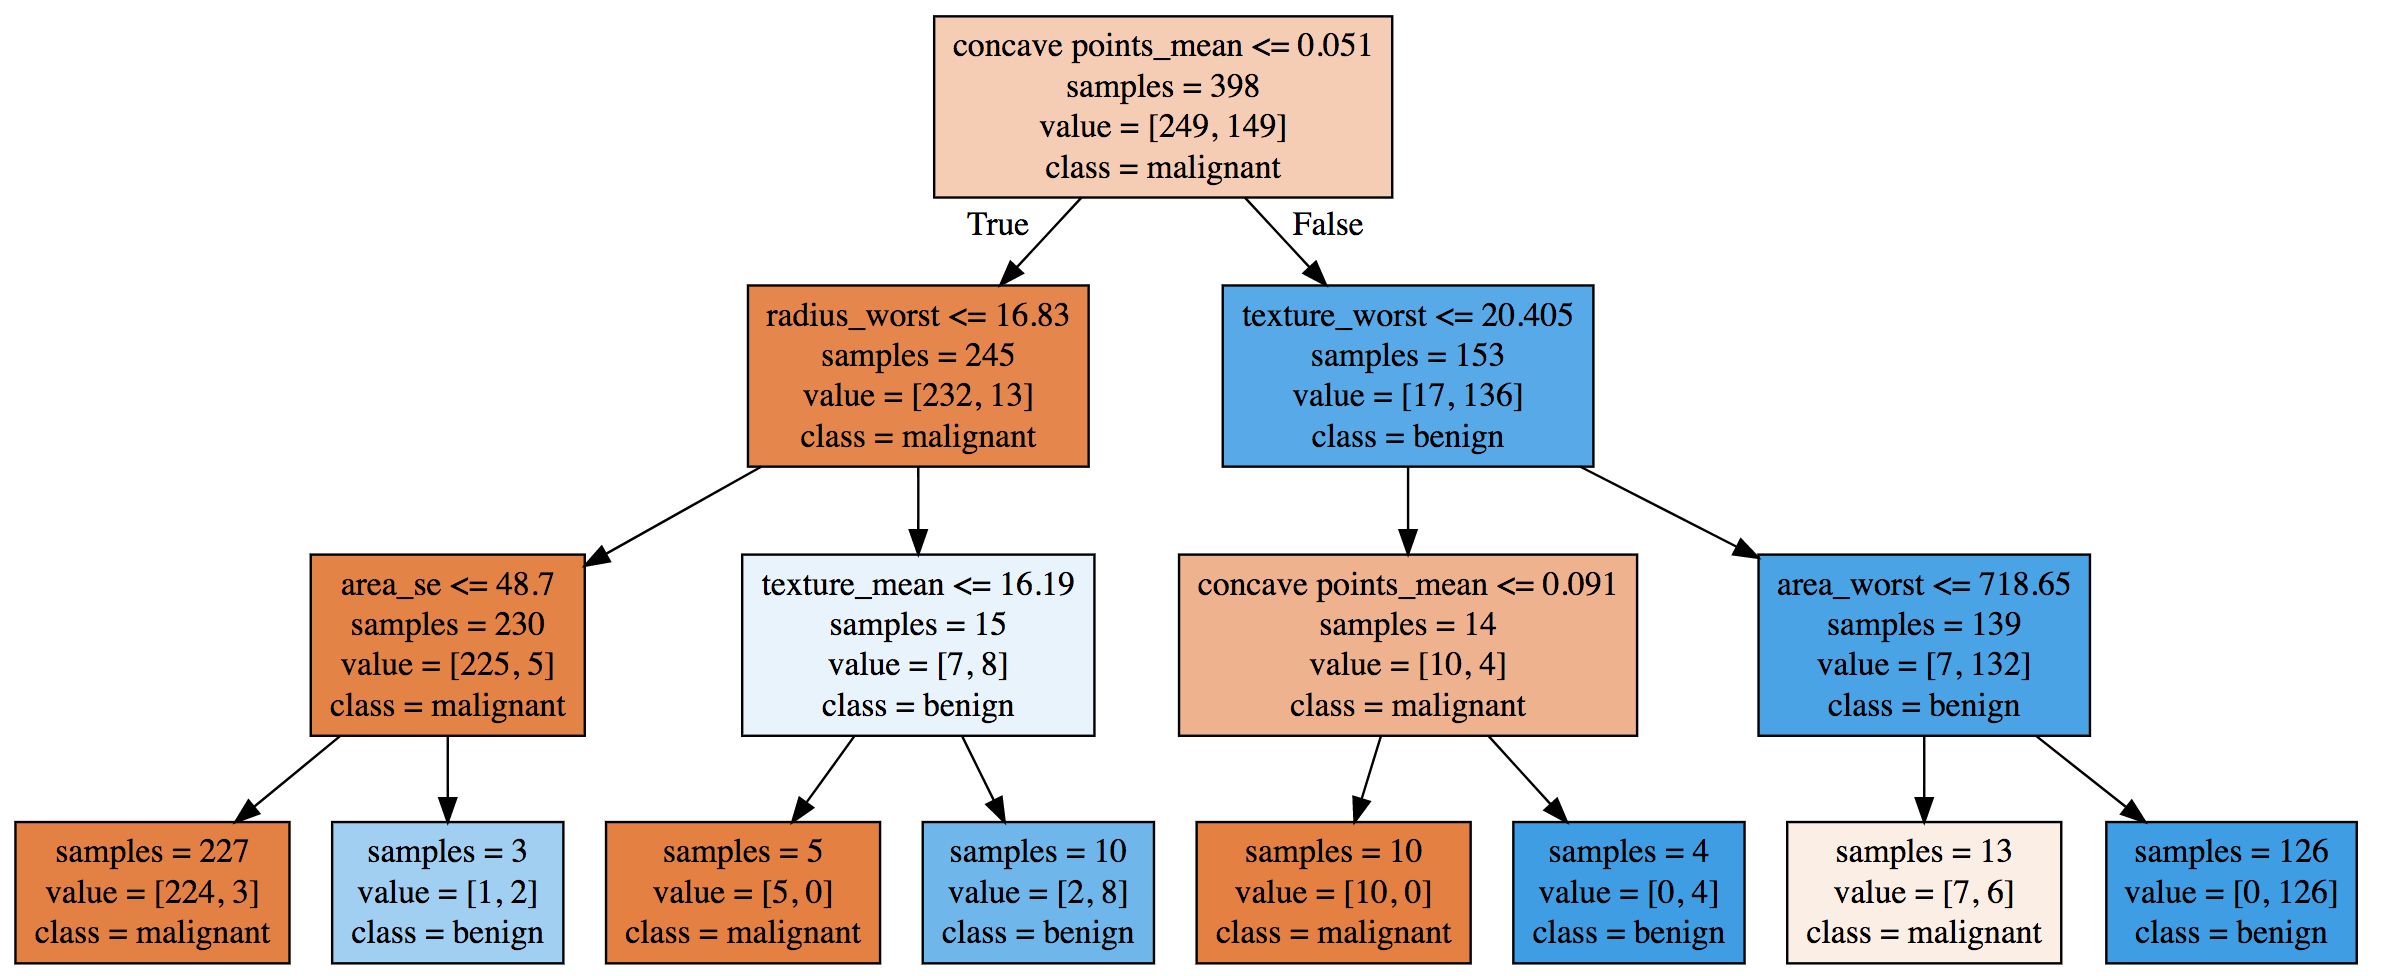
\includegraphics[width=\textwidth]{graphviz}
	\caption{Representation of the decision tree built on the dataset}
	\label{fig:graphviz}
\end{figure}

As \cref{fig:graphviz} is limited to the certain depth of 3, bigger and more deep trees can be really over whelming and hard to grasp. So it's always better to display the trees after doing some pruning or pre-pruning. In this task in order to control the model complexity and preventing it from overfitting, we have applied a pre-pruning by changing both \emph{$max\_depth$} parameter and \emph{$max\_leaf\_nodes$} parameter and the results are presented in \cref{fig:DT_maxdepth} and \cref{fig:DT_maxleafnodes} respectively. 

\begin{figure}[h]
    \centering
    \begin{subfigure}{0.45\textwidth}
        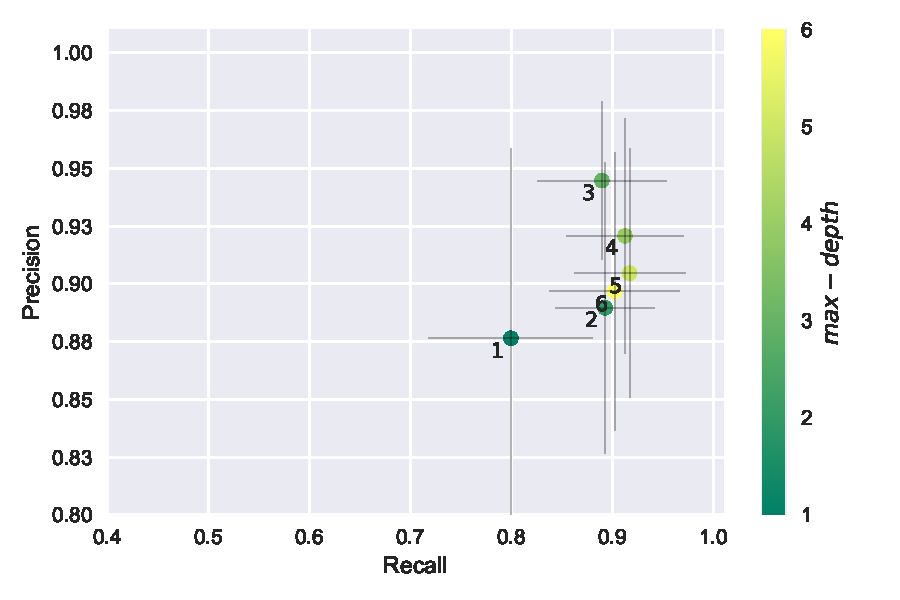
\includegraphics[width=\textwidth]{prec_recall_dt_maxdepth}
        \caption{}
        \label{fig:prec_recall_dt_maxdepth}
    \end{subfigure}
    \begin{subfigure}{0.45\textwidth}
        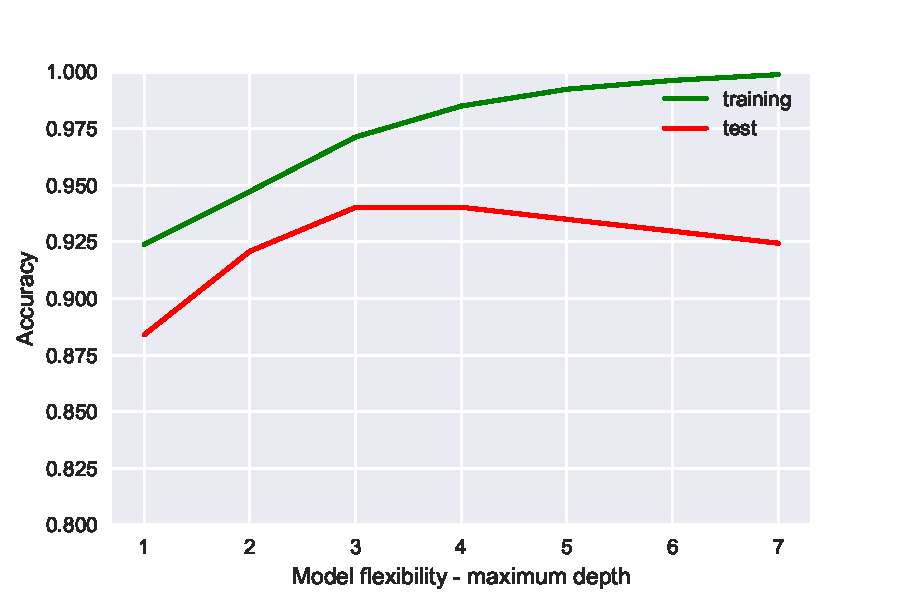
\includegraphics[width=\textwidth]{tradeoff_dt_maxdepth}
        \caption{}
        \label{fig:tradeoff_dt_maxdepth}
    \end{subfigure}
    \caption{Decision Tree classifier output with different maximum depth values, (a) precision-recall plot (b) Trade-off of model flexibility against training and test accuracy}\label{fig:DT_maxdepth}
\end{figure}

\begin{figure}[h]
    \centering
    \begin{subfigure}{0.45\textwidth}
        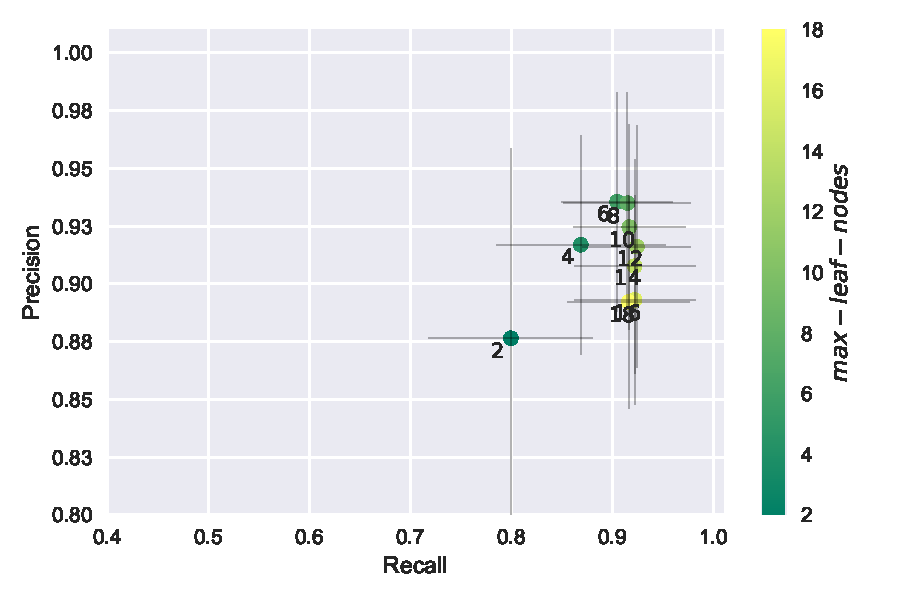
\includegraphics[width=\textwidth]{prec_recall_dt_maxleafnodes}
        \caption{}
        \label{fig:prec_recall_dt_maxleafnodes}
    \end{subfigure}
    \begin{subfigure}{0.45\textwidth}
        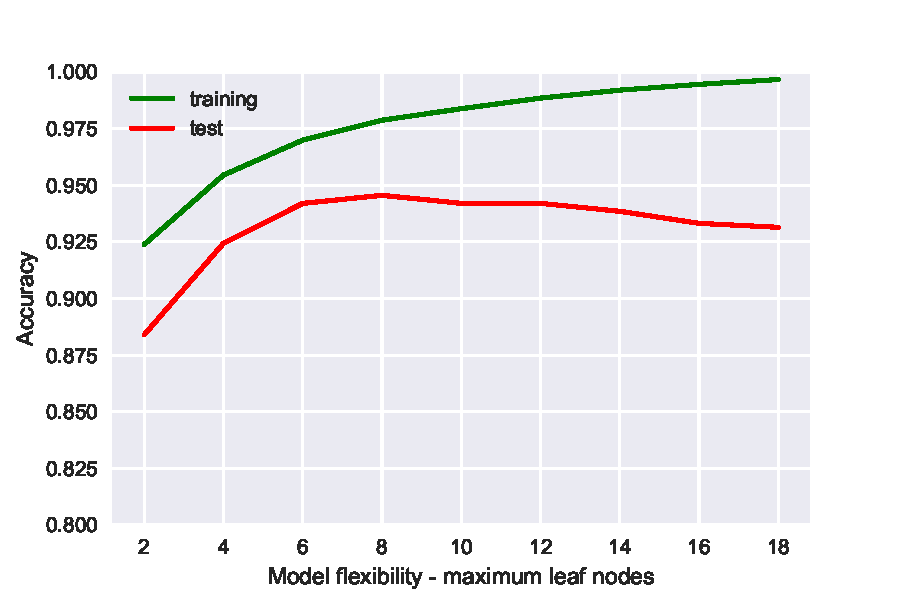
\includegraphics[width=\textwidth]{tradeoff_dt_maxleafnodes}
        \caption{}
        \label{fig:tradeoff_dt_maxleafnodes}
    \end{subfigure}
    \caption{Decision Tree classifier output with different maximum leaf nodes values, (a) precision-recall plot (b) Trade-off of model flexibility against training and test accuracy}\label{fig:DT_maxleafnodes}
\end{figure}

As it's being presented in \cref{fig:DT_maxdepth}, assigning a maximum depth of 3 would result in best test performance and prevent the classifier from overfitting the prediction on test set, and it is actually the reason behind visualizing the tree in \cref{fig:graphviz} with the mentioned depth. The results are:

\begin{align*}
	\text{accuracy} &= 0.94 \pm 0.025 \\
	\text{precision} &= 0.92 \pm 0.05 \\
	\text{recall} &= 0.91 \pm 0.06 \, .
\end{align*}

later we'll show performing methods of ensembles of trees, like Random Forests would lower the overfitting and enhance the prediction.
Taking a closer look at \cref{fig:graphviz} shows certain paths in the trees are contributing the most in the classification task. For example, looking at branches to the left of the tree, and following along the branch which ends in the very left leaf node of the tree, will show that 227 of samples has been classified on this path. Very similar to such a path can be found on the right hand side of the tree ending up with 126 of the samples inside it. 

Looking into such paths may imply another parameter in which would be important in interpreting the decision trees. This parameter is an indicator of how much a features is contributing in the classification process.  Takin another look into \cref{fig:graphviz} on the node on the very left of the tree containing 230 samples, although it contains a considerable amount of the samples, but applying the $area\_se \leq 48.7$ only extract 3 samples to the benign class and the remaining 227 samples are still in the malignant class which would imply that \emph{$area\_se$} is a less contributing feature in classification task, comparing to for instance \emph{$texture\_mean$} feature, which extracts 5 malignant samples out of 15 benign ones. Feature importance can be drawn for all the features of the dataset by the same concept, and it is a value between zero and one, one being the most contributing and zero being no contribution at all. These values are calculated for this dataset and is shown in \cref{fig:feature_importance}. Important to notice is that, although in this tree, the higher features in the tree hierarchy has more importance than the lower one, but this is not always the case and it is because as discussed in \cref{sec:theo}, the splitting process is \emph{greedy}.

\begin{figure}[h]
	\centering
	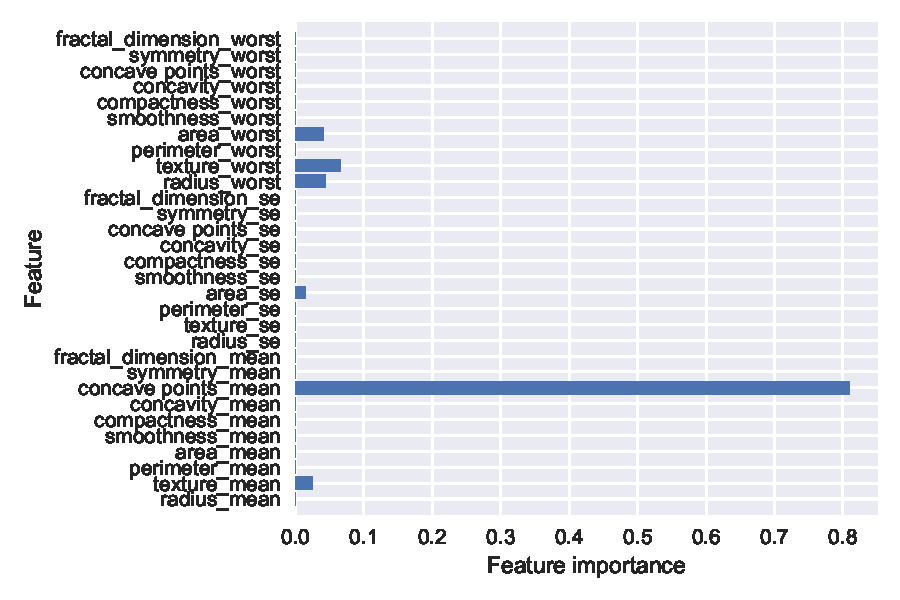
\includegraphics[width=.6\textwidth]{feature_importance}
	\caption{Feature importance on the decision tree implemented for the dataset}
	\label{fig:feature_importance}
\end{figure}

Important to notice that low feature importance does not necessarily mean that the feature is uninformative, but it only means that the tree has not chose it, probably because another feature encoding the same information \citep{muller2016introduction}. There are many features which have zero importance and that is because the tree has the depth of 3, which means only 7 ($1+2+4$) features has the chance to contribute in the tree and these were the best fit. Of course having deeper trees would result in more features contributing in the tree, or as we metioned in \cref{sec:theo}, random forest would exploit much more number of features, due to it's random feature selection, coming in next section.

\paragraph{Random Forests (AN)} The random forests model gets it's power from the different decision trees it exploits. A parameter which can be set in it's class in Scikit Learn module. Applying the classifier in different number of decision trees would make the process of tuning the classifier possible. Results are showed in \cref{fig:RF}.

\begin{figure}[h]
    \centering
    \begin{subfigure}{0.45\textwidth}
        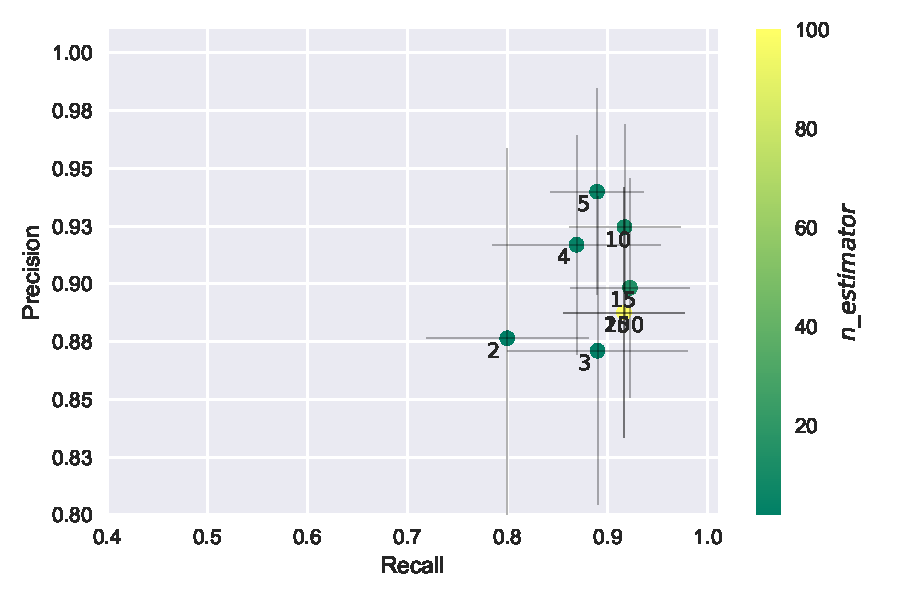
\includegraphics[width=\textwidth]{prec_recall_rf}
        \caption{}
        \label{fig:prec_recall_rf}
    \end{subfigure}
    \begin{subfigure}{0.45\textwidth}
        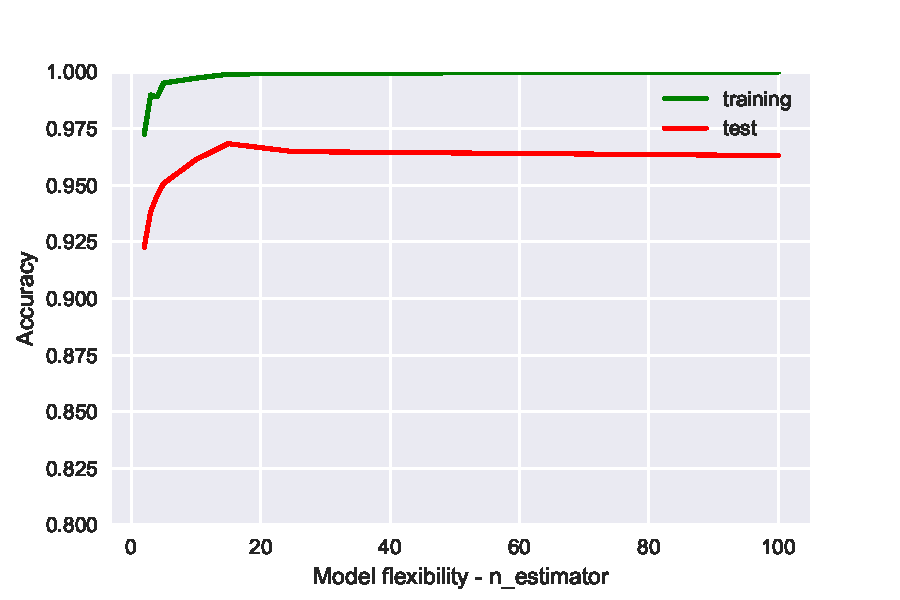
\includegraphics[width=\textwidth]{tradeoff_rf}
        \caption{}
        \label{fig:tradeoff_rf}
    \end{subfigure}
    \caption{Random Forests classifier output for different number of trees, (a) precision-recall plot (b) Trade-off of model flexibility against training and test accuracy}\label{fig:RF}
\end{figure}

we are observing an enhance in our test prediction right away from taking even 4 or 8 trees in our model. This means random forests model overfits less than any decision tree individually. We are achieving the same what a fine tuned decision tree did with 4 trees and with out any pruning or pre-pruning(Note that pruning and pre-pruning is possible in Random Forests models and it may achieve in better results, depends on the dataset). The best results are scored with 15 trees:

\begin{align*}
	\text{accuracy} &= 0.968 \pm 0.015 \\
	\text{precision} &= 0.97 \pm 0.025 \\
	\text{recall} &= 0.947 \pm 0.028 \, .
\end{align*}

Note that random forests models usually uses lot more trees, in hundreds or even thousands, however, we have achieved the same accuracy for thousand trees, with a simple model of 15 ones. This shows how random forests are robust to overfitting and adding more trees wouldn't deteriorate the results anyhow. 

As we were expecting in a random forest model, much more features will contribute in the classification task, and that is due to the random feature selection routine embedded in this model, resulting in much more informative feature importance, depicted in \cref{fig:feature_importance_rf}.

\begin{figure}[h]
	\centering
	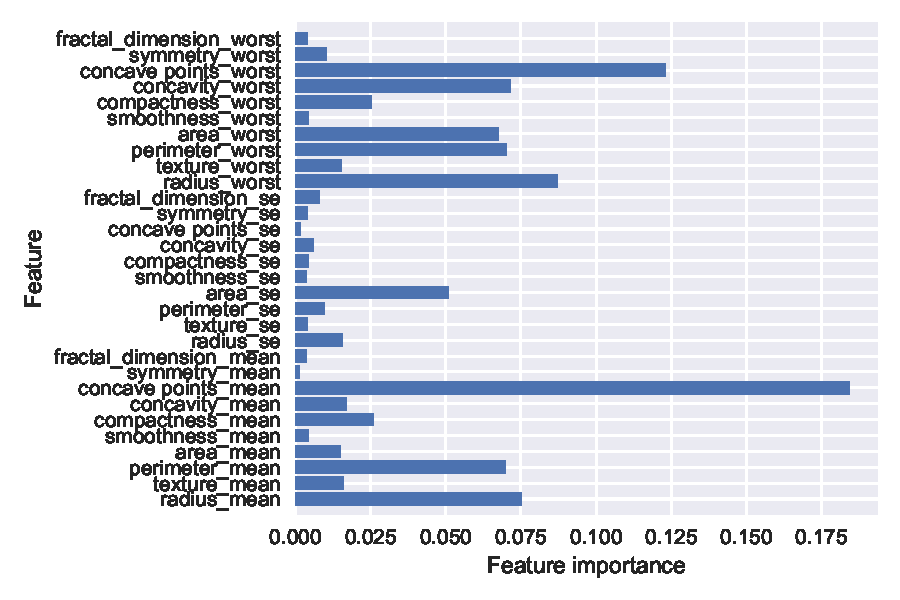
\includegraphics[width=.6\textwidth]{feature_importance_rf}
	\caption{Feature importance on the random forest implemented for the dataset}
	\label{fig:feature_importance_rf}
\end{figure}

Noteworthy to add that one can tune the parameters for random forest by adjusting \emph{$max\_features$} parameter, however setting it to \emph{auto} would normally result in the same results, more or less.

\paragraph{(k-)Nearest Neighbor (JK).} The cross-validated precision-recall results for the k-NN classifier can be seen in \cref{fig:knn1}. Most generally, the classifier achieves very good performance on the data set.
As is usually expected, an initial increase in the $k$ number of neighbors considered in the majority vote increases the performance of classification as this helps stabilize the prediction against outliers. However, when too many neighbors are considered, the predictive power of the classifier should decrease, since neighbors that are too far away, and are therefore likely to be of a different class, contribute to the majority vote. One can weigh the votes of each neighbor by the inverse of the distance from the instance to classify to somewhat remedy this problem.

The best performance is achieved at $k=9$ with 
\begin{align*}
	\text{accuracy} &= 0.97 \pm 0.02 \\
	\text{precision} &= 0.99 \pm 0.03 \\
	\text{recall} &= 0.93 \pm 0.05 \, .
\end{align*}
However the high noise from the cross-validation makes it entirely possible that other $k$ might achieve better performance on other test sets. However, their performance will most likely be very similar to the one achieved with $k=9$, i.e.\  it does not really matter.

In this data set, we notice that the precision value of the classifier increases by 4 percentage points as we go to a 2-NN classifier. However, afterwards the data set is almost indifferent to an increase in $k$.  The recall value does slightly increase, however not significantly w.r.t.\ the standard deviation. This stability against $k$ at the fact that meaningful features exist, clustering the data in a stable manner and therefore an increase in $k$ does not decrease the score.\footnote{As $k$ is increased, eventually instances of the opposite class are considered in the majority vote. However, if the data is approximately spherically clustered, an increasing number of correct instances is also considered. Therefore meaningful features yield some stability against large values of $k$.}
Only as we increase $k$ to large values of $k>50$ can a decrease in precision be observed, and finally the classifier breaks down at extreme and absolutely unreasonable $k$, i.e.\  the recall value increases because a lot of the positive instances are being falsely misclassified as negatives, because the data set is imbalanced (more negative than positive instances) and at high $k$ this leads to a lot of false negatives, because the algorithm simply predicts the majority class. If the classification is redone with an artificially balanced data set the recall value at high $k$ does not exhibit this behavior as heavily.

However, at reasonable $k$ the imbalance in the data set does not affect the performance of the k-NN classifier, which makes sense, because imbalance is a global quantity whereas the k-NN classifier only looks at local balls in feature space.
\begin{figure}
	\centering
	 \begin{subfigure}[b]{0.45\textwidth}
	 	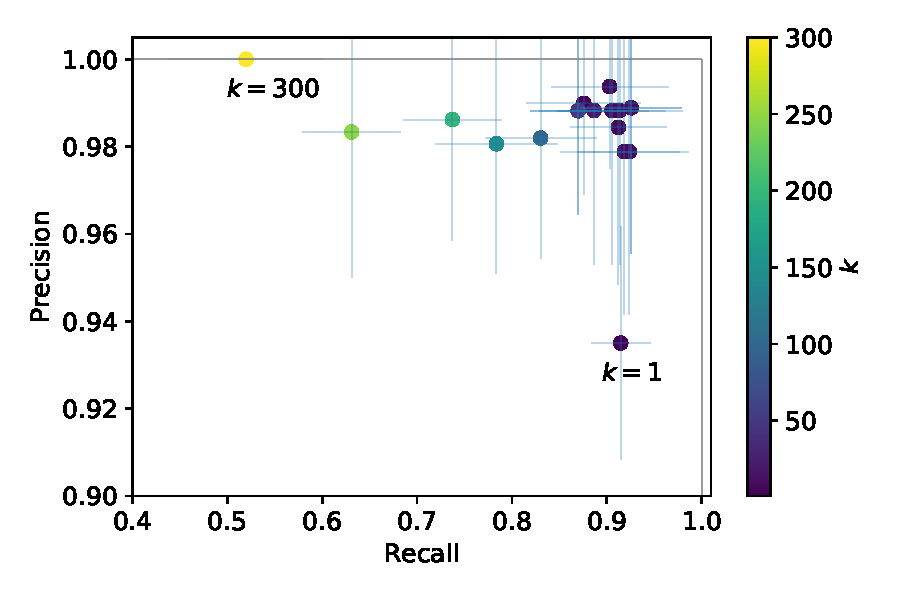
\includegraphics[width=\textwidth]{knn}
	 	\caption{}
	 	\label{fig:knn1}
    \end{subfigure}
	 \begin{subfigure}[b]{0.45\textwidth}
	 	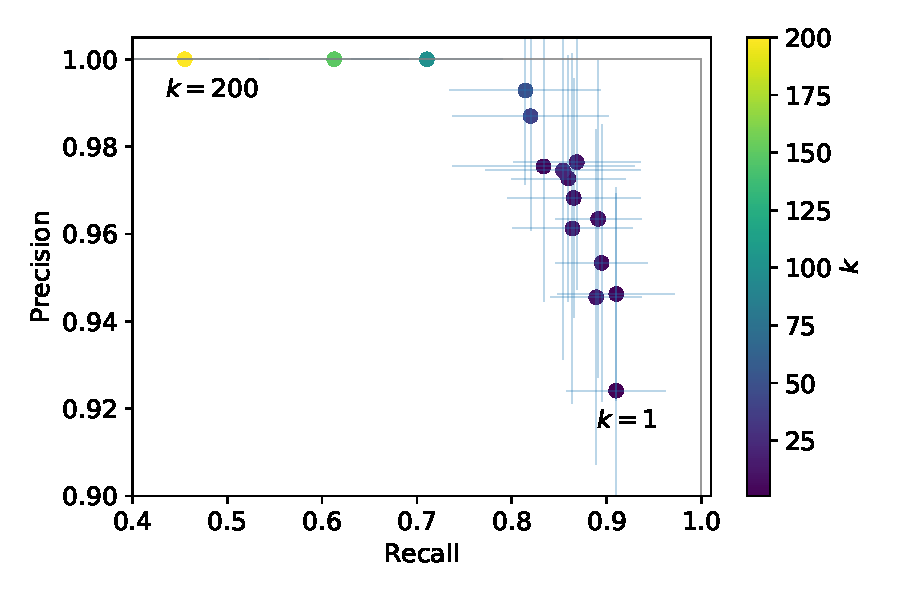
\includegraphics[width=\textwidth]{knn_pca}
	 	\caption{}
	 	\label{fig:knn2}
    \end{subfigure}
	\caption{Precision-recall plot of the k-NN classifier for different values of k in the (a) original feature space and (b) the first four dimensions of the PCA. The grey line represents an ideal classifier.}
	\label{fig:knn}
\end{figure}

The k-NN algorithm has also been applied to the first four components of the PCA, which explain about \SI{80}{\percent} of the variance of the original data. A few differences can be achieved. Firstly, the performance of the PCA k-NN stays slightly below the performance of the raw k-NN. This is relieving, as our data set does not contain a lot of instances ($\approx 600$) in a space of 30 dimensions. One could have thought that the performance of the classifier in the original feature breaks down due to the \emph{curse of high dimensions}. Compare to \cite{barber2012brm, bishop2006prm} for a textbook discussion of the topic.
Intuitively as the number of dimensions rises, the volume of a hypercube rises exponentially and therefore an exponential number of points are needed to cover the space densely. This means that high-dimensional data can very easily get sparse. It also affects the Euclidean distance metric: at high dimensions, the distance from one point to all its neighbors becomes very similar. Even though  space is sparsely populated, most of the points are concentrated at a similar distance. 
This is why the raw k-NN precision-recall curve seems to bunch together all $k\in \{2,\dots, 20\}$ while the PCA k-NN precision-recall curve is more spread out. In high dimensions, as we increase the number of neighbors taken into consideration, we do not actually venture further away from the point. Therefore, the points on the precision-recall curve are bunched together, except for extreme values of $k$. The expected effect of increasing k (smooth curve with optimum at some $k$, and bad performance at extremal values) can only be observed for low dimensional data.
There is some discussion in the literature to what extend the performance of k-NN and related algorithms is necessarily affected by dimensionality. However, this is beyond the scope of this report and the reader is referred to \cite{marimont1979nearest, Chavez01searchingin, paper3}.

\paragraph{Support Vector Machines (JK).} The SVM was successfully applied to the data set. The results of the linear SVM can be taken from \cref{fig:svm1}. Compared to the nearest neighbor algorithm, the linear SVM shows an interesting behavior as the trade-off parameter $C$ is increased. As $C$ is increased from small values, both precision and recall increase somewhat linearly until an optimal value is reached, from which the classifier then decays in a similar way as $C$ is increased further.

The optimal value of
\begin{align*}
	\text{accuracy} &= 0.98 \pm 0.01 \\
	\text{precision} &= 0.99 \pm 0.01 \\
	\text{recall} &= 0.96 \pm 0.03 \
\end{align*}
is reached at $C = 0.04$. As discussed in \cref{sec:theo}, low $C$ values express a preference of maximizing the margin and allowing misclassification in the training set. However, this shall not be over-interpreted as the results for higher $C$ values yield similar performance when accounting for uncertainty in the values.

While at first glance the performance of this classification is better than the scores obtained by simpler classification algorithms such as the NN, it has to be noted that the noise in the results does not allow such conclusions. It seems that in our comparison between the algorithms we are fundamentally limited by said noise in our data set. While one can speculate that an increase in sample size might help, it could be that the noise is simply inherent to the data, i.e.\ the quality of the features inherently limits the classification performance.

\begin{figure}
	\centering
	 \begin{subfigure}[b]{0.45\textwidth}
	 	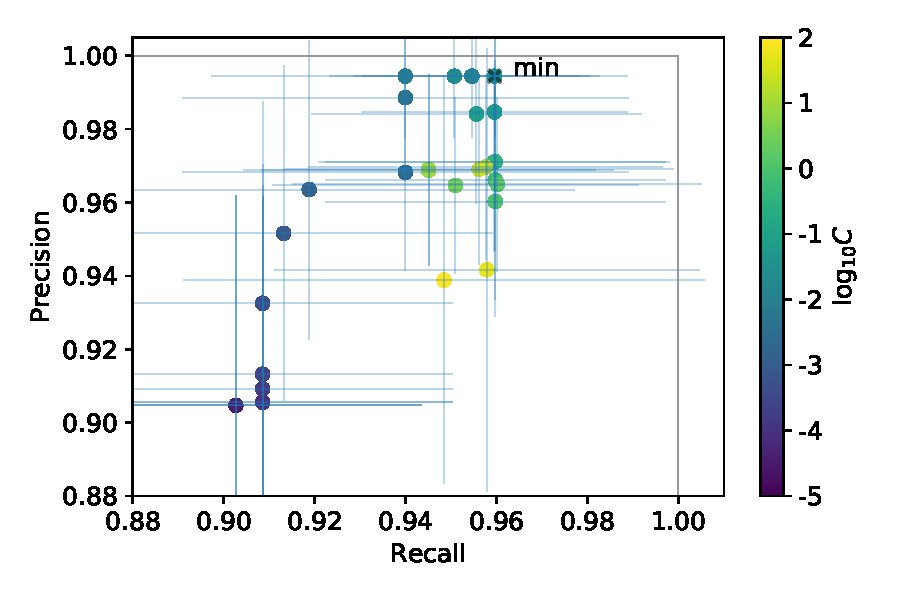
\includegraphics[width=\textwidth]{svm}
	 	\caption{}
	 	\label{fig:svm1}
    \end{subfigure}
	 \begin{subfigure}[b]{0.45\textwidth}
	 	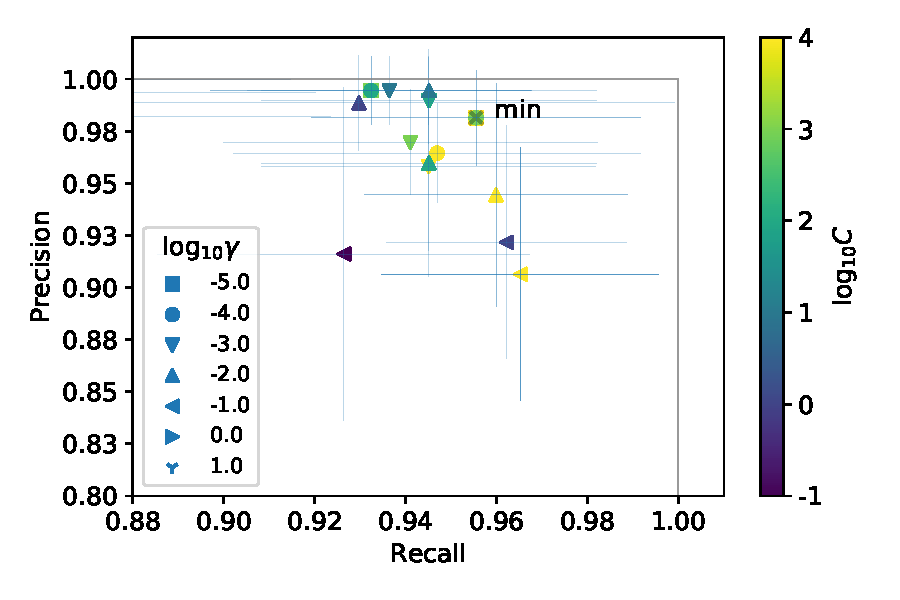
\includegraphics[width=\textwidth]{svm_grid}
	 	\caption{}
	 	\label{fig:svm2}
    \end{subfigure}
	\caption{Precision-recall plot of the SVM classifier for different values of (a) the trade-off parameter $C$ for a linear SVM and (b) a grid of values $C$ and $\gamma$ for a kernelized SVM with a Gaussian kernel.}
	\label{fig:svm}
\end{figure}

Again, the artificially balanced data set did not result in better classifier performance. Although SVMs can suffer from undesired results when the data is imbalanced, this does not occur here in any way noticeable.

A kernel SVM with a Gaussian kernel was also applied and a grid search performed over possible combinations of $C$ and the kernel parameter $\gamma$.
The resulting cross-validated precision-recall curve for this grid search can be seen in \cref{fig:svm2}.
There is no consistently apparent behavior of the precision-recall curve as either $C$ or $\gamma$ are varied. This is likely due to the fact that, limited by the computational complexity, the grid search only searches through orders of magnitudes for the desired parameters and therefore the variations in the classification behavior cannot be observed. A second round of grid search could have been performed after the first one, if the uncertainty in the data were lower and results at such resolution meaningful.

The best result, acknowledging that this is just a \emph{trend} and that the noise in the cross-validation is too high, was achieved at $(C=10^3, \gamma=10^{-4})$ with
\begin{align*}
	\text{accuracy} &= 0.98 \pm 0.02 \\
	\text{precision} &= 0.96 \pm 0.03 \\
	\text{recall} &= 0.98 \pm 0.02 \, .
\end{align*}
Again, the errors do not permit any detailed comparison between other algorithms, though it seems that the limited complexity of the data set is already well accounted for by a simple linear SVM. Note that for some extreme values not shown in the plot, e.g.\ low $C$ or high $\gamma$, the classification performance breaks down completely.

\paragraph{Multilayer Perceptron (JK).} Neural networks have many hyperparameters such as learning rate (How much do we adjust the parameters after each backpropagation?), batch size (How many instances do we feed into the network before we backpropagate?), epochs(How many times do we propagate all of the data through the network?), as well as the general architecture of the network (How deep is the network, how many neurons per layer, what kind of non-linearity, ...?). Additionally, training large neural networks is computationally expensive, which is why grid searches over the hyperparameter space as well as cross-validation are rarely seen in current publications.\footnote{Plus, in this report, I see the MLP more as a pet project, a nice little extra, whose performance need not to be pushed to the maximum.}

A simple MLP with \SI{30} input nodes, \SI{300} nodes in a single hidden layer, and \SI{2} output nodes was constructed. Training for \SI{200} epochs with \SI{50} instances per batch and a learning rate of \SI{0.05} yielded a test set performance of 
\begin{align*}
	\text{accuracy} &= 0.98 \\
	\text{precision} &= 0.97  \\
	\text{recall} &= 0.98  \, .
\end{align*}
However, due to the reasons mentioned above no cross validation was performed, and the values are therefore without error. Due to the stochastic nature of the batch training, the values vary slightly between different sessions. However, even though no hyperparameter optimization was performed, the test set classification performance of a simple MLP is fairly high and comparable the other presented algorithms.

\section{Discussion}
\label{sec:discu}

%TODO unfortunately original images are not available. otherwise could have trained CNN to do it all automatically just like thorsten did in his paper
%TODO essentially not comparable with the high noise present
%TODO read up, there was some way to make cross validation less noisy, that we could have used


\section{Summary}
\label{sec:sum}

%TODO most / all? our algorithms reached performance atleast par with what original authors published


\bibliographystyle{ieeetr}
\bibliography{bibliography}

\end{document}
